\problemname{Islands in the Data Stream}

Given a sequence of integers $a_1, a_2, a_3, \ldots, a_n$, an island in the
sequence is a contiguous subsequence for which each element is greater
than the elements immediately before and after the subsequence.  In the
examples below, each island in the sequence has a bracket below it.
The bracket for an island contained within another island is below the
bracket of the containing island.

\begin{figure}[!h]
\begin{center}

\includegraphics[]{b1.png} \\
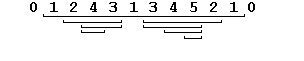
\includegraphics[]{b2.png} \\

\includegraphics[]{b3.png} \\
\end{center}
\end{figure}

Write a program that takes as input a sequence of $12$ non-negative
integers and outputs the number of islands in the sequence.

\section*{Input}

The first line of input contains a single integer $P$, ($1 \le P \le 1000$),
which is the number of data sets that follow.  Each data set should be
processed identically and independently.

Each data set consists of a single line of input.  It contains the
data set number, $K$, followed by $12$ non-negative integers separated by
a single space.  The first and last integers in the sequence will be 0.


\section*{Output}

For each data set there is one line of output.  The single output line
consists of the data set number, $K$, followed by a single space followed
by the number of islands in the sequence.
